\documentclass[12pt, a4]{article}
\usepackage[english]{babel}
\usepackage[utf8x]{inputenc}
\usepackage{fullpage}
\usepackage{listings}
\usepackage{graphicx}
\usepackage{color}

%Syntax highlighting
\definecolor{blue-violet}{rgb}{0.54, 0.17, 0.89}
\definecolor{ao}{rgb}{0.0, 0.5, 0.0}
\definecolor{amaranth}{rgb}{0.9, 0.17, 0.31}
\definecolor{ballblue}{rgb}{0.13, 0.67, 0.8}
\definecolor{onyx}{rgb}{0.06, 0.06, 0.06}


\lstset{
  breaklines=true,                 % automatic line breaking only at whitespace
  captionpos=b,                    % sets the caption-position to bottom
  breakatwhitespace=false,
  keepspaces=true,
  numbers=left,
  numbersep=5pt,
  showspaces=false,
  showstringspaces=false,
  showtabs=false,
  tabsize=4,  
  backgroundcolor=\color{white},   % choose the background color
  commentstyle=\color{ao},    % comment style
  keywordstyle=\color{amaranth},    % keyword style
  stringstyle=\color{blue-violet},    % string literal style
  numberstyle=\tiny\color{ballblue},	   % number style
  basicstyle=\ttfamily\footnotesize\color{onyx} % size of fonts used for the code
}

%Document Header
\title{\textbf{Department of CSE\\SSN College of Engineering}}
\author{\textbf{Vishakan Subramanian - 18 5001 196 - Semester VII}}
\date{19 July 2021}

\begin{document}
\maketitle
\hrule
\section*{\center{UCS 1711 - Mobile Application Development Lab}}
\hrule
\bigskip

%Assignment Details
\subsection*{\center{\textbf{Exercise 1: Application Using GUI Components, Font and Colours}}}
\subsection*{\flushleft{Aim:}}
\begin{flushleft}
Generate a registration form for a hospital to register new patient details as below:

\begin{itemize}
\item Assign a title for the registration form(TextView- textSize, textStyle , typeface)
\item Name. Specify some font and colour. (use TextView, EditText-standard)
\item Address (use TextView, EditText-standard)
\item Age (TextView, EditText)
\item Date of Birth (DatePicker)
\item Gender (RadioButton)
\item Marital Status (Spinner)
\item Contact Number (EditText- inputType, phoneNumber)
\item Registration time (TimePicker)
\item Addiction (Smoking, Alcohol) (CheckBox)
\item Submit (Button)
\item Reset (Button)

\end{itemize}
\end{flushleft}

%Code
\newpage
\subsection*{\flushleft{Code: Main Activity:}}
\begin{flushleft}
\lstinputlisting[language = Java]{PatientRegistration/app/src/main/java/com/example/patientregistration/MainActivity.java}
\end{flushleft}

%Code
\newpage
\subsection*{\flushleft{Code: Submit Activity}}
\begin{flushleft}
\lstinputlisting[language = Java]{PatientRegistration/app/src/main/java/com/example/patientregistration/SubmitActivity.java}
\end{flushleft}

%Code
\newpage
\subsection*{\flushleft{Code: Main Activity Layout}}
\begin{flushleft}
\lstinputlisting[language = XML]{PatientRegistration/app/src/main/res/layout/activity_main.xml}
\end{flushleft}

%Code
\newpage
\subsection*{\flushleft{Code: Submit Activity Layout}}
\begin{flushleft}
\lstinputlisting[language = XML]{PatientRegistration/app/src/main/res/layout/activity_submit.xml}
\end{flushleft}


%Output
\newpage
\subsection*{\flushleft{Output: Empty Form:}}
\begin{figure}[h]
\centering
\caption{Output: Empty Form.}
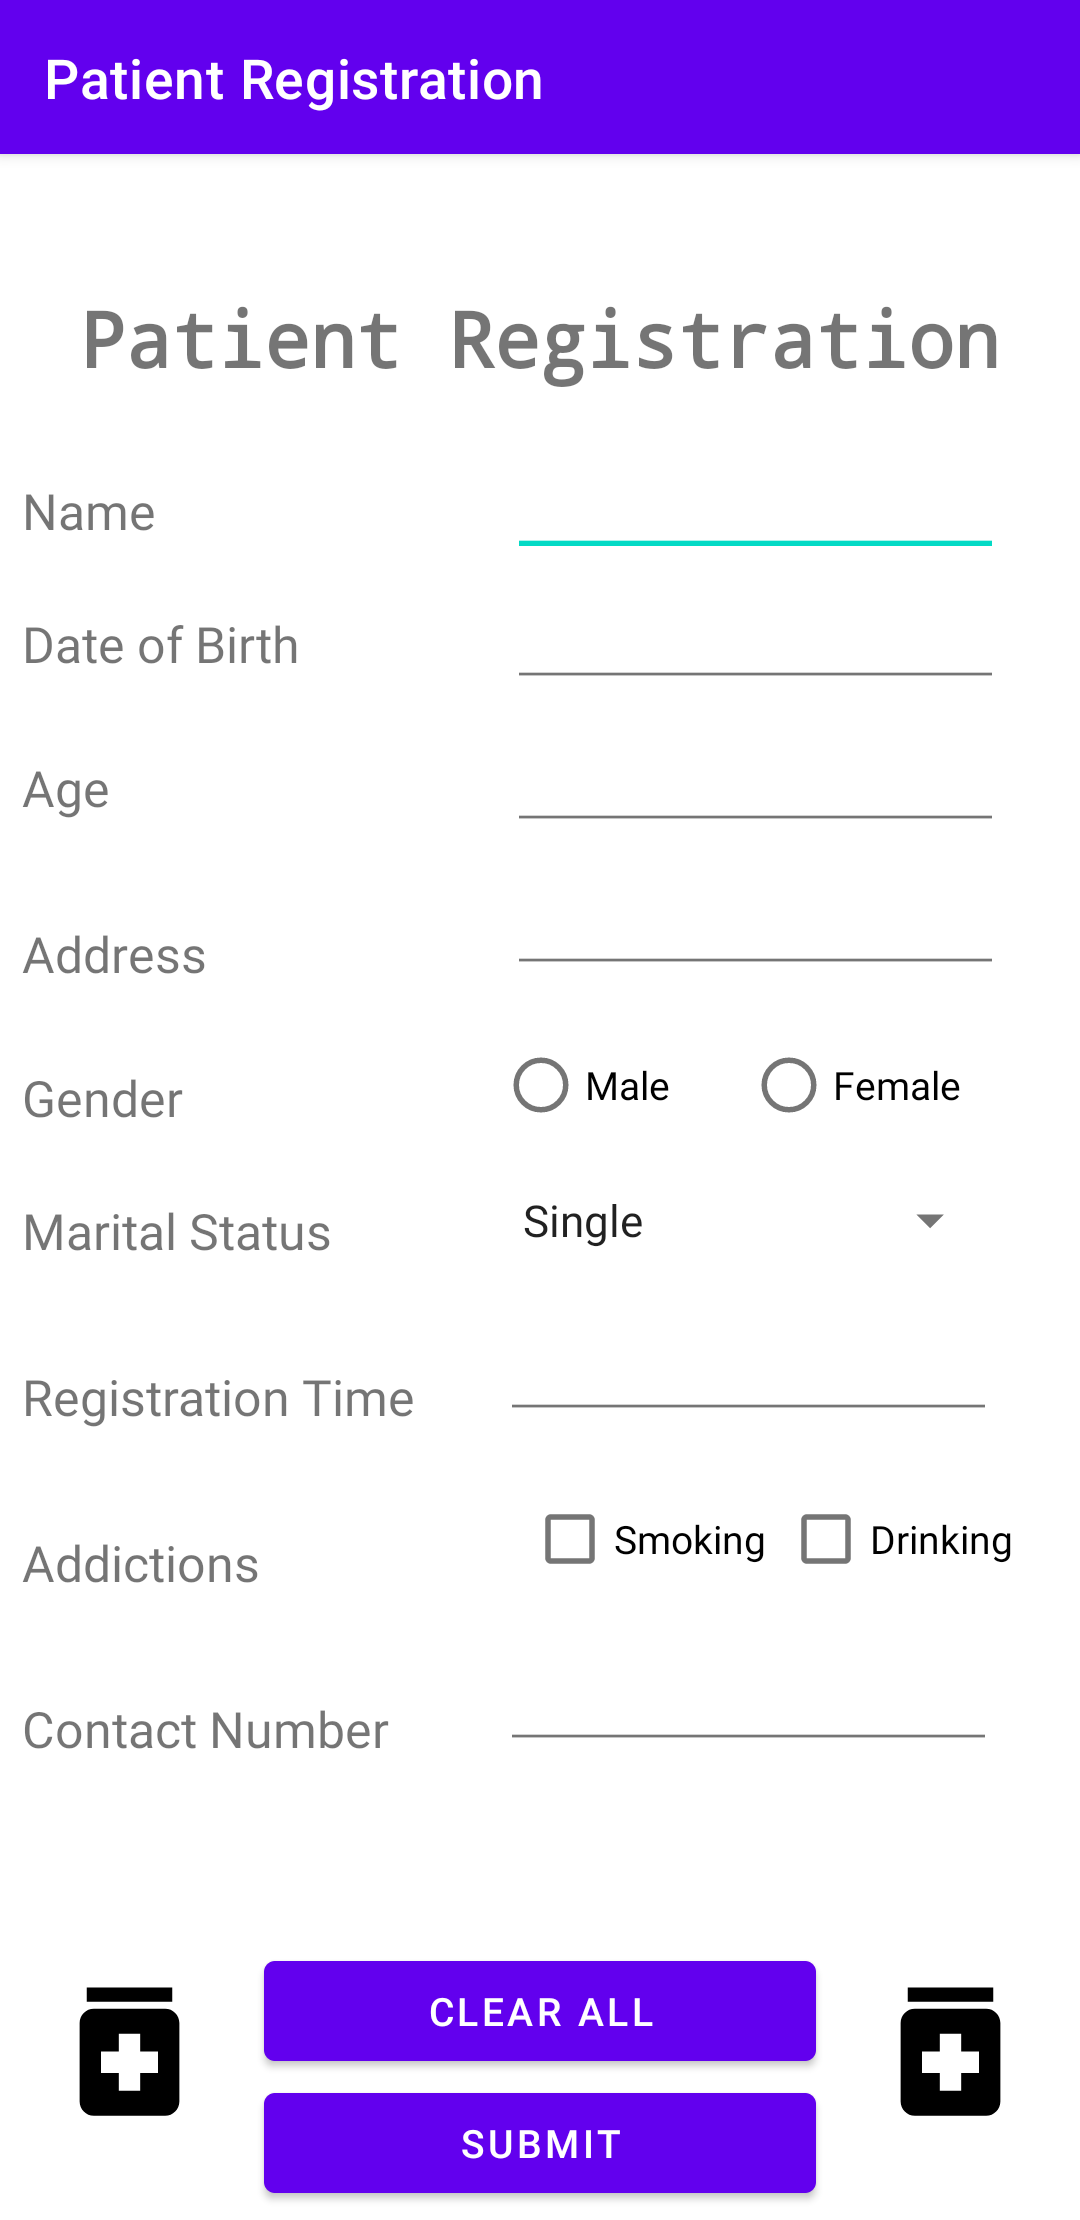
\includegraphics[height=15cm, width=7.3cm]{PatientRegistration/Screenshots/EmptyForm.png}
\end{figure}

%Output
\newpage
\subsection*{\flushleft{Output: Filled Form:}}
\begin{figure}[h]
\centering
\caption{Output: Filled Form.}
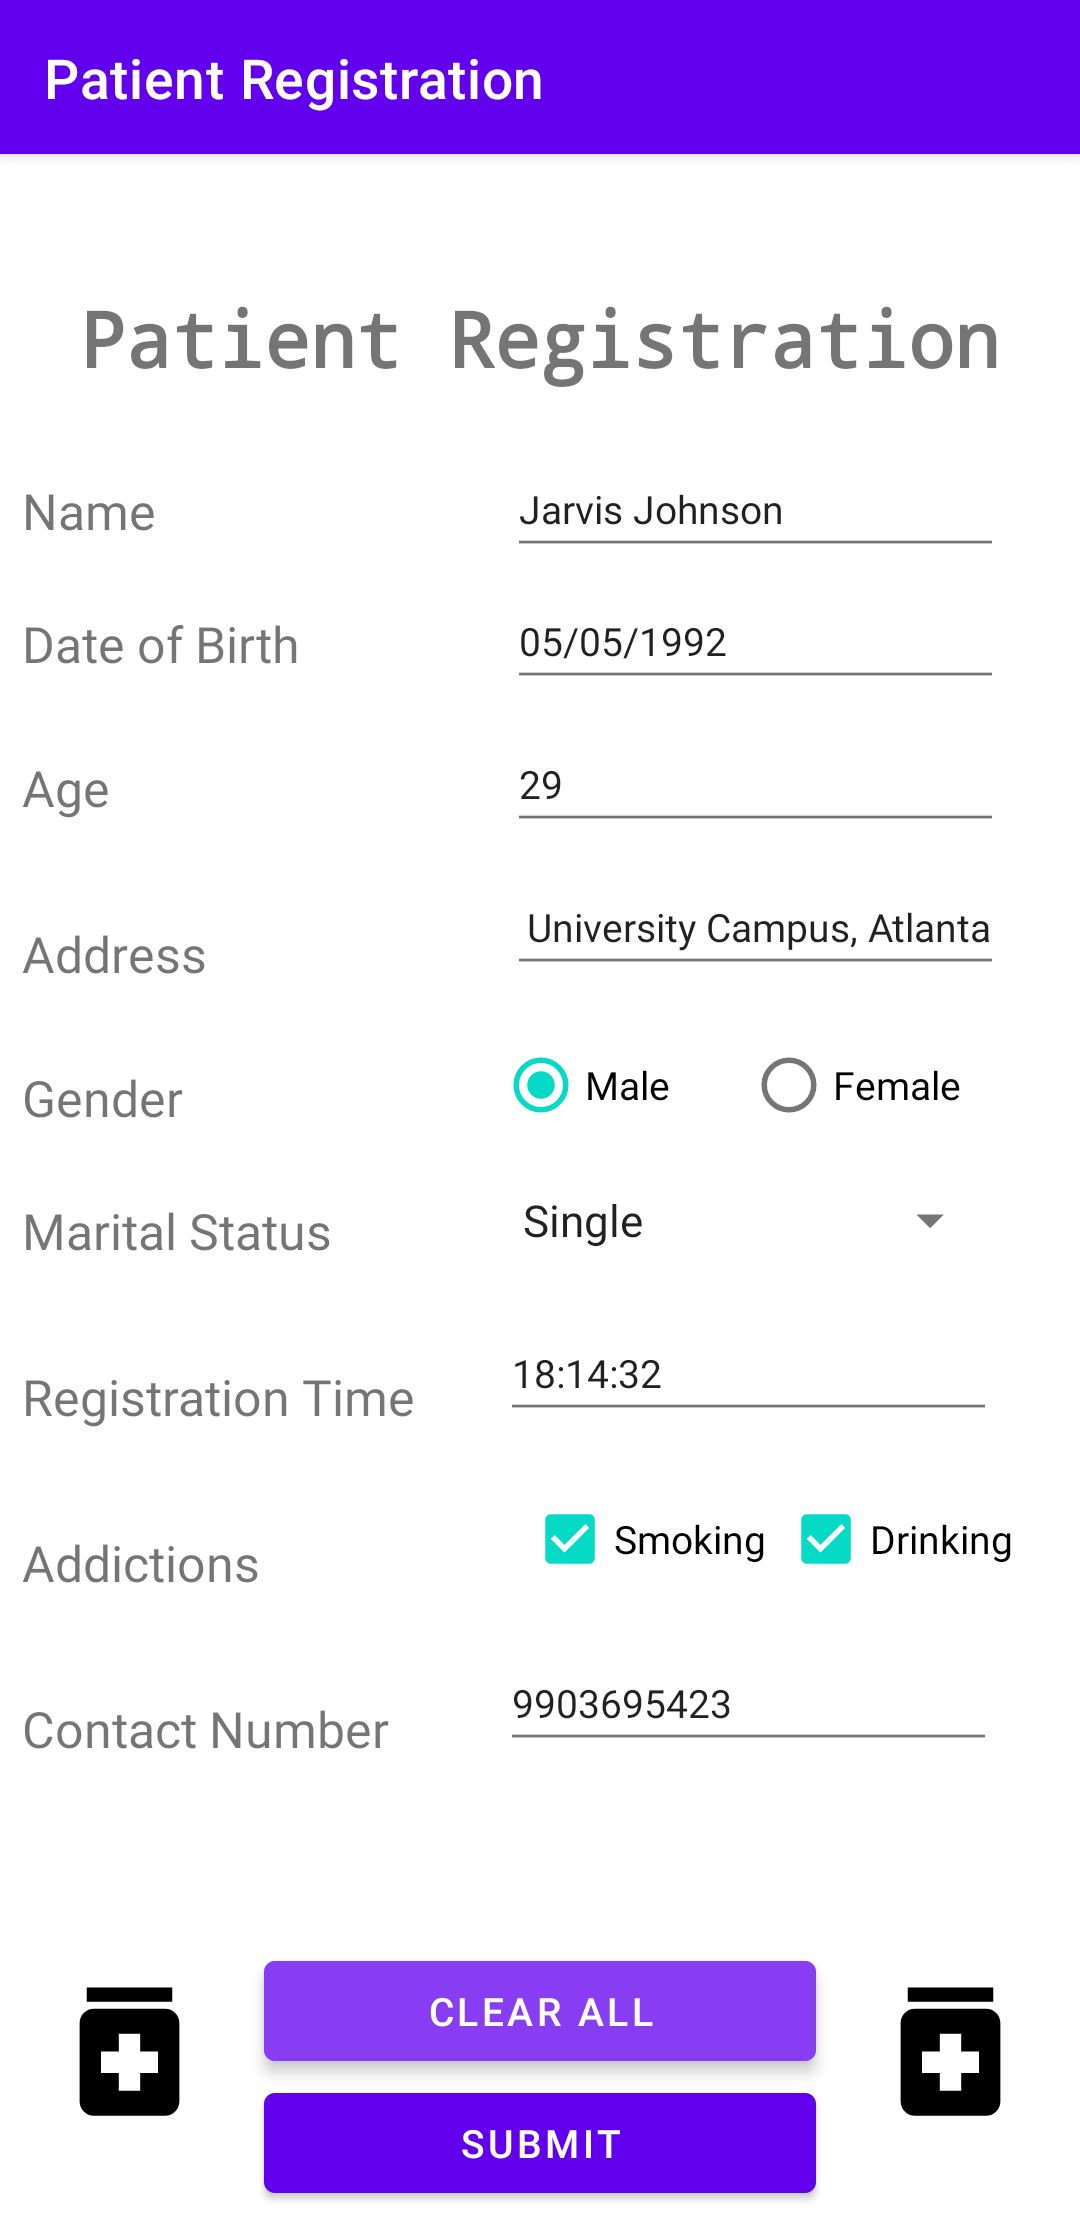
\includegraphics[height=15cm, width=7.3cm]{PatientRegistration/Screenshots/FilledForm.png}
\end{figure}

%Output
\newpage
\subsection*{\flushleft{Output: Submitted Form:}}
\begin{figure}[h]
\centering
\caption{Output: Submitted Form.}
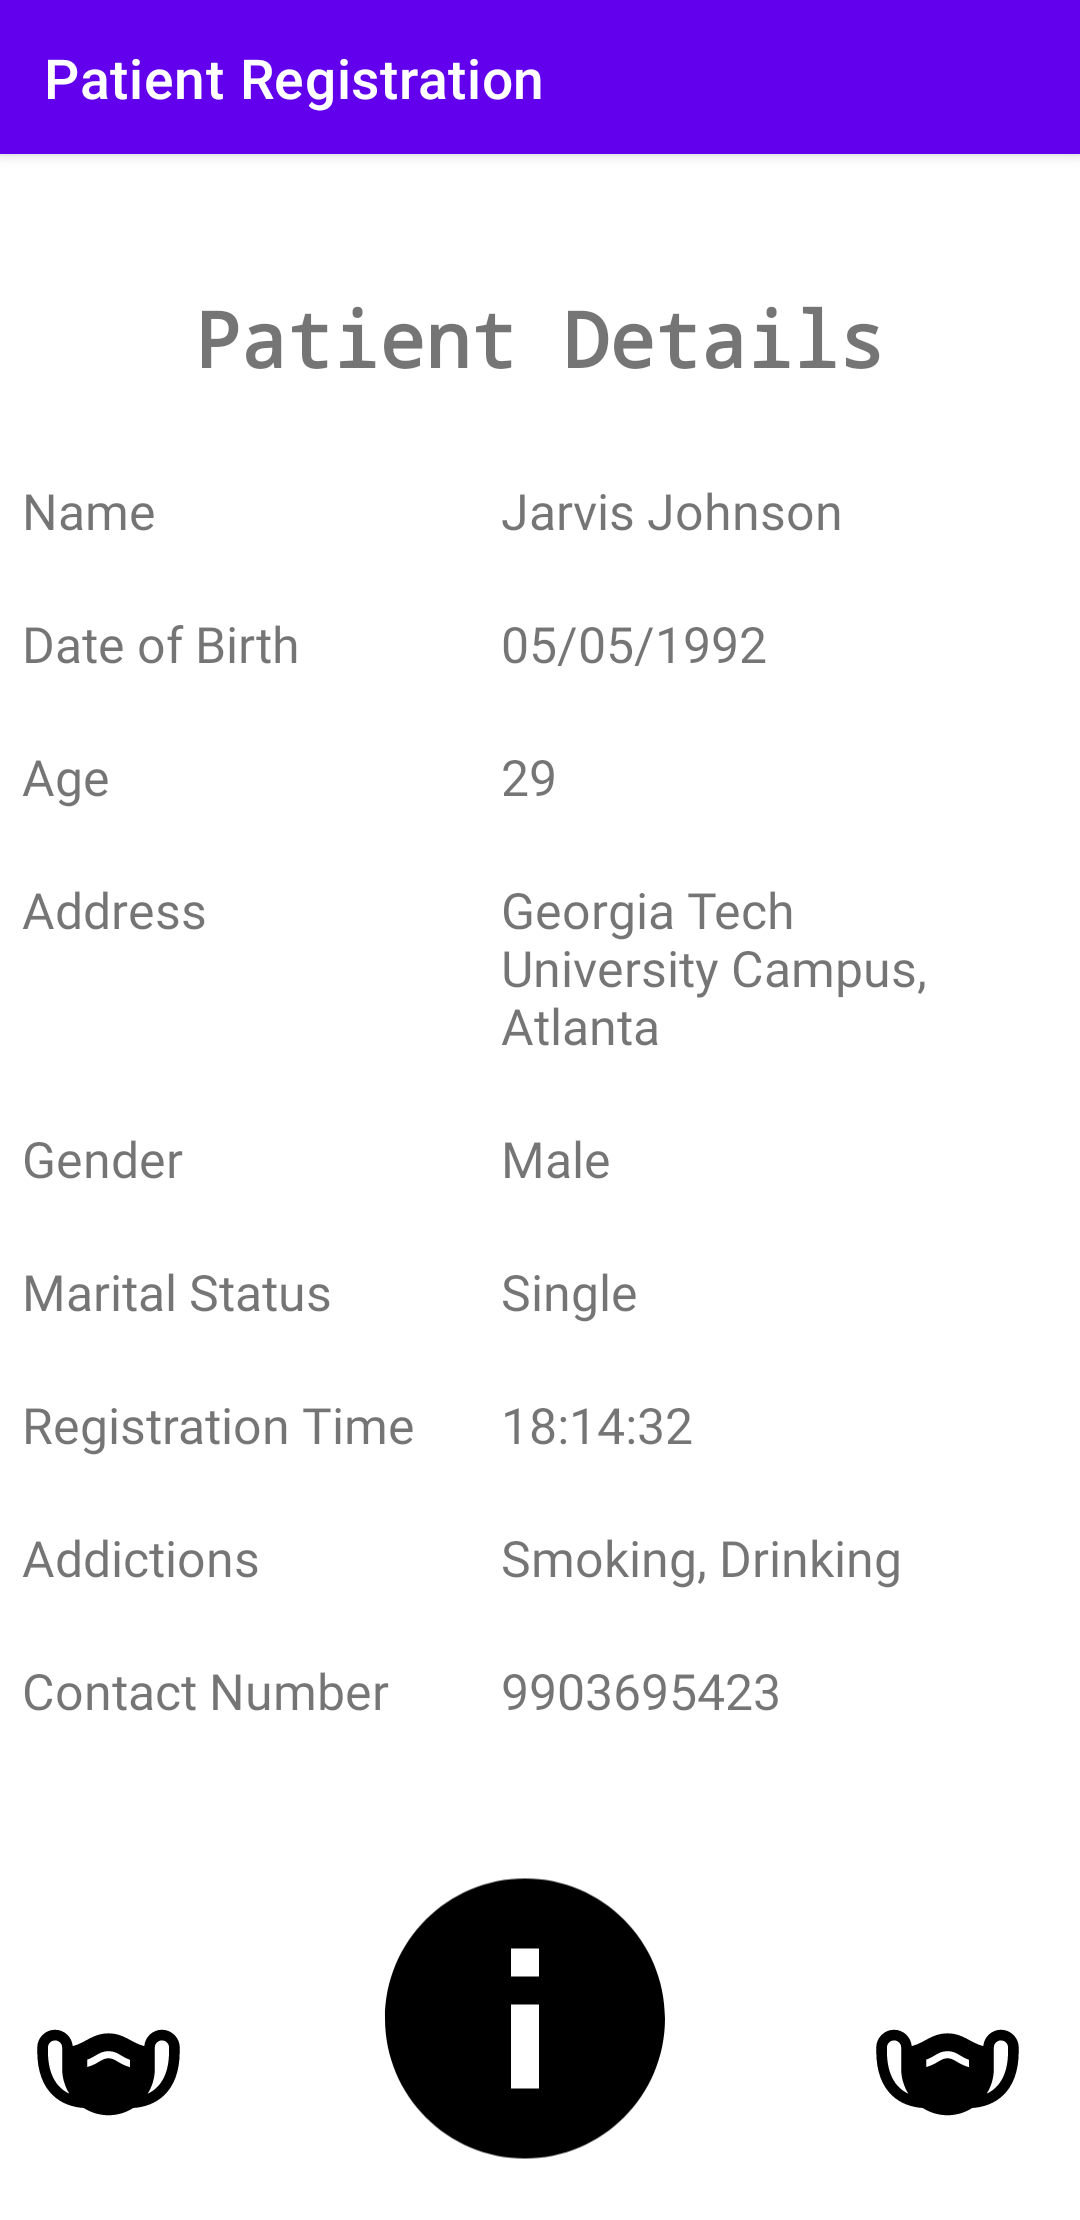
\includegraphics[height=15cm, width=7.3cm]{PatientRegistration/Screenshots/SubmittedForm.png}
\end{figure}

%Learning Outcome
\newpage
\subsection*{\flushleft{Learning Outcome:}}
\begin{itemize}
\item I was able to install \textbf{Android Studio IDE} and create a new project.
\item I understood how to code a simple form with \textbf{GUI components} using Java and XML.
\item I understood how to use the design window to design the front-end GUI layout without requiring to write XML code to do the same.
\item I used multiple GUI components like \textbf{TextView, ImageView, Button, PlainText, Phone, PostalAddress, Number, RadioButton, CheckBox, RadioGroup, Date \& Time}.
\item I understood how to use \textbf{Constraint Layout} for basic front-end development.
\item I understood how the usage of \textbf{Spinner} to create a drop-down list and I was able to populate it with a custom-defined list with the help of \textbf{strings.xml}
\item I implemented \textbf{onClickListener} events to the buttons to perform required form actions.
\item I understood the usage of \textbf{Intent} to transfer data from one Activity to another.
\item I understood how to call a new Activity from existing Activity using the help of Intent.
\item I was able to store and extract form data using Intent and display it on a new Activity.
\item I configured different \textbf{font styles, font sizes and colors} for different UI elements with the element's design attributes.
\item I was able to develop and run a basic \textbf{Android application} on my computer and also export it to my phone as an \textbf{APK file} and use it from my mobile device.
\end{itemize}


\end{document}